\documentclass{beamer}
\usepackage{Presentacion}

\title[Detección de Deadlocks en Rust]{Detección de Deadlocks en Rust \\ en tiempo de compilación \\ mediante Redes de Petri}
\author{Horacio Lisdero Scaffino}
\institute[FIUBA]{Facultad de Ingeniería\\Universidad de Buenos Aires}
\date{19 de febrero del 2023}
% TWEAK THE FONT SIZE
\setbeamerfont{date}{size=\scriptsize}
% ADD LOGO
\logo{
\includegraphics[height=1.3cm]{FIUBA-Logo.png}}

\AtBeginSection[]
{
  \begin{frame}{Agenda}
  \footnotesize
    \tableofcontents[currentsection, currentsubsection]
  \end{frame}
}

\AtBeginSubsection[]
{
  \begin{frame}{Agenda}
  \footnotesize
    \tableofcontents[currentsection, currentsubsection]
  \end{frame}
}

\begin{document}

\begin{frame}
  \titlepage
\end{frame}

% REMOVE THE LOGO FROM NOW ON %
\logo{}

\begin{frame}{Agenda}
  \tableofcontents
\end{frame}

\section{Introducción}

\begin{frame}{Una vista general de la herramienta}
  El traductor es el componente principal.
  El verificador de modelos y el compilador de Rust, \emph{rustc}, son dependencias.

  \begin{figure}
    \centering
    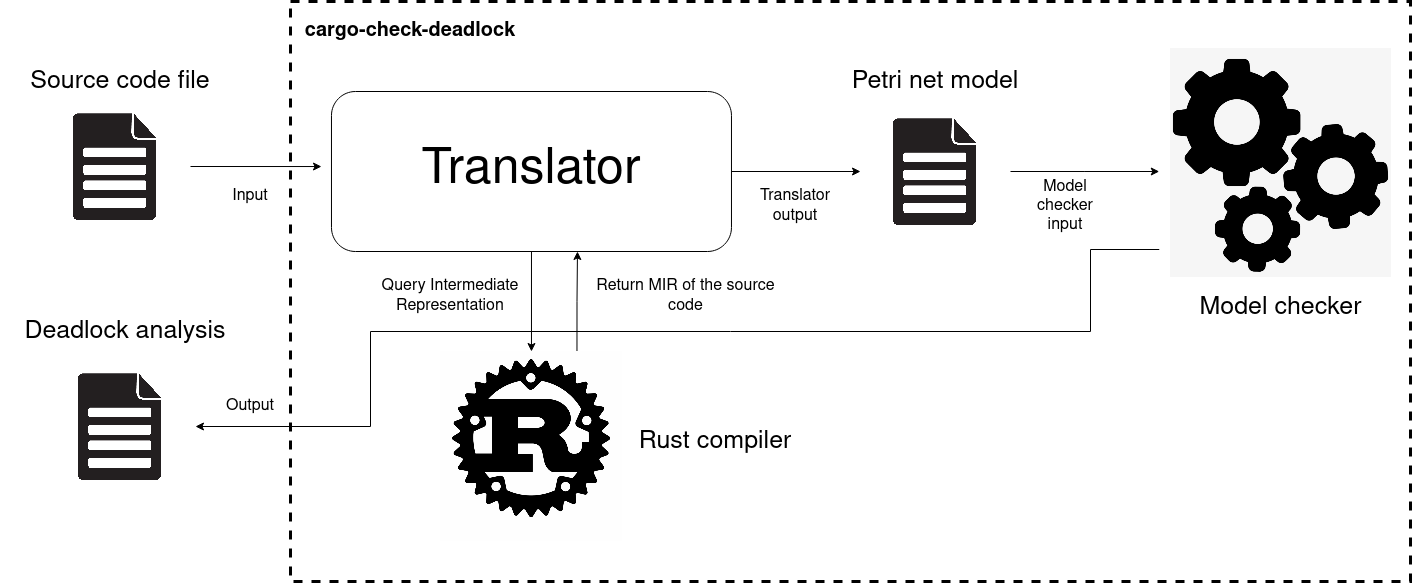
\includegraphics[width=\linewidth]{cargo-check-deadlock-logic-view.png}
  \end{figure}
\end{frame}

\section{Rust}

\subsection{¿Qué es Rust?}

\begin{frame}{¿Qué es Rust?}
  Rust es un lenguaje de programación multiparadigma de uso general que
  busca ofrecer a los desarrolladores una forma segura y eficiente de escribir código de bajo nivel.
  
  \pause
  \vfill

  \begin{itemize}
    \item Uso seguro de la memoria (\emph{Memory safe})
    \item Compilado a código máquina, con un \emph{runtime} mínimo
    \item Expresividad de un lenguaje de alto nivel
    \item Performance de un lenguaje de bajo nivel (similar a C o C++)
  \end{itemize}
\end{frame}

\begin{frame}{Breve línea de tiempo de Rust}
  \begin{description}
    \item [2007] Inicio como un proyecto personal de Graydon Hoare, un programador en Mozilla
    \item [2009] Mozilla comienza a patrocinar oficialmente el proyecto
    \item [2015] Primera versión estable 1.0
    \item [2016] Mozilla lanza Servo, un motor de navegador construido con Rust
    \item [2019] Se estabiliza el soporte de \Rustinline{async}/\Rustinline{await}
    \item [2021] AWS, Huawei, Google, Microsoft y Mozilla crean la Rust Foundation.
    \item [2021] El proyecto Android fomenta el uso de Rust para los componentes del SO por debajo del ART
    \item [2022] El kernel de Linux añade soporte para Rust junto con C
    \item [2023] 8 años consecutivos el lenguaje de programación más querido en la Stack Overflow Developer Survey
  \end{description}
\end{frame}

\begin{frame}{Uso seguro de la memoria}
  Logra un uso seguro de la memoria sin recurrir a un recolector de basura o a un contador de referencias.
  En su lugar, utiliza el concepto de \textbf{ownership} (propiedad) y \textbf{borrowing} (préstamo).

  \vfill

  Evita una gran variedad de clases de errores en tiempo de compilación:

  \begin{itemize}
    \item Double free
    \item Use after free
    \item Punteros colgantes (\emph{Dangling pointers})
    \item Condiciones de carrera (\emph{Data races})
    \item Pasaje de variables no seguras entre hilos
  \end{itemize}

  \vfill

  Si se encuentra una violación de las reglas del compilador, el programa simplemente no compilará.
\end{frame}

\subsection{¿Por qué Rust?}

\begin{frame}{El uso seguro de la memoria es fundamental para la fiabilidad y la seguridad}
  Investigaciones empíricas han concluido que alrededor del 70\% de las vulnerabilidades encontradas en
  grandes bases de código en C/C++ se deben a errores de gestión de memoria.
  Esta elevada cifra puede observarse en proyectos como:

  \begin{itemize}
    \item Android Open Source Project \cite{memory-bugs-android},
    \item los componentes Bluetooth y multimedia de Android \cite{memory-bugs-android-media-bluetooth},
    \item el Proyecto Chromium detrás del navegador web Chrome \cite{memory-bugs-chrome},
    \item el componente CSS de Firefox \cite{memory-bugs-firefox},
    \item iOS y macOS \cite{memory-bugs-ios-macos},
    \item productos de Microsoft \cite{miller-security-microsoft2019, memory-bugs-microsoft},
    \item Ubuntu \cite{memory-bugs-ubuntu}
  \end{itemize}
\end{frame}

\begin{frame}{La adopción de Rust aumenta velozmente}
  \scriptsize
  \begin{itemize}
    \item El proyecto Android Open Source fomenta
          el uso de Rust para los componentes del SO
          por debajo del ART \cite{stoep2021}.
    \item El kernel Linux versión 6.1 introduce soporte oficial de las herramientas
          para programar componentes en Rust \cite{corbet2022,desimone2022}.
    \item En Mozilla, el proyecto Oxidation se creó en 
          para aumentar el uso de Rust en Firefox y aplicaciones relacionadas. 
          En marzo de 2023, las líneas de código en Rust representan
          más del 10\% del total en Firefox Nightly \cite{mozilla-oxidation}.
    \item En Meta, el uso de Rust como lenguaje de desarrollo \emph{server-side}
          está aprobado y se fomenta desde julio de 2022 \cite{garcia2022}.
    \item En Cloudflare, se construyó desde cero un nuevo proxy HTTP en Rust
          para superar las limitaciones arquitectónicas de NGINX,
          reduciendo el uso de CPU en un 70\% y el uso de memoria en un 67\% \cite{wu2022}.
    \item En Discord, reimplementar un servicio crucial
          en Rust proporcionó grandes beneficios de performance
          y solucionó un problema ligado a la recolección de basura en Go \cite{howarth2020}.
    \item En npm Inc, la empresa detrás del registro npm,
          Rust permitió escalar los servicios ligados a la CPU
          a más de 1300 millones de descargas diarias \cite{rust-npm-case-study}.
    \item Un estudio del código basado en Rust descubrió que se ejecuta tan eficientemente
          que consume la mitad de electricidad que un programa similar escrito en Java,
          un lenguaje de uso común en AWS \cite{pereira2017energy}.
  \end{itemize}
\end{frame}

\begin{frame}{Las herramientas son modernas y fáciles de usar}
  \begin{itemize}
    \item \href{https://doc.rust-lang.org/stable/cargo/}{cargo},
          el gestor de paquetes oficial: Formatear, compilar, testear, lint, actualizar y publicar paquetes.
    \item \href{https://doc.rust-lang.org/book/ch11-00-testing.html}{Test harness}
          para pruebas unitarias, pruebas de integración y pruebas en comentarios de documentación (doctests).
          No se necesitan bibliotecas de terceros.
    \item Un registro público oficial para los paquetes Rust (llamados ``crates''): \url{https://crates.io/}.
    \item Generación automática de un sitio web estático a partir de los comentarios en el código del proyecto.
          Se publica automáticamente en \url{https://docs.rs/}.
    \item Un linter oficial incluido en la instalación por defecto que detecta aún más errores
          y detecta código no idiomático: \href{https://github.com/rust-lang/rust-clippy}{clippy}.
    \item La integración con git, GitHub, VSCode, IntelliJ es excelente y fácil de usar.
    \item Una nueva versión estable del compilador cada 6 semanas \cite{albini2019}.
  \end{itemize}
\end{frame}

\section{Redes de Petri}

\subsection{¿Qué es una red de Petri?}

\begin{frame}{Definición informal}
  Una red de Petri es una herramienta de modelado matemático
  utilizada para describir y analizar el comportamiento de sistemas concurrentes.
  Proporciona una representación gráfica del estado del sistema y sus transiciones,
  permitiendo el análisis visual y formal de procesos complejos.

  \begin{figure}[!htb]
    \centering
    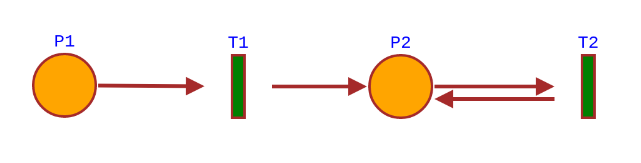
\includegraphics[width=0.8\linewidth]{petri-net-formal-example.png}
  \end{figure}

  \scriptsize
  \begin{itemize}
    \item Lugares: Representan estados en el sistema (\emph{circles})
    \item Transiciones: Representan eventos o acciones que ocurren en el sistema (\emph{rectángulos}).
    \item Tokens: Marcas dentro de lugares que son creadas
          y consumidas por las transiciones (\emph{puntos dentro de lugares})
  \end{itemize}

  \vfill
\end{frame}

\begin{frame}{Definición matemática}
  Una red de Petri es una 5-tupla, $ PN = (P, T, F, W, M_{0}) $ donde:

  \begin{quote}
    $ P = \{ p_1, p_2, \dots, p_m \} $ es un conjunto finito de lugares,\\
    $ T = \{ t_1, t_2, \dots, t_n \} $ es un conjunto finito de transiciones,\\
    $ F \subseteq (P \times T) \cup (T \times P) $ es un conjunto de arcos (relación de flujo),\\
    $ W: F \rightarrow \{1, 2, 3, ... \} $ es una función de peso para los arcos,\\
    $ M_{0}: P \rightarrow \{0, 1, 2, 3, .... \} $ es el marcado inicial,\\
    $ P \cap T = \varnothing $ y $ P \cup T \neq \varnothing $
  \end{quote}
  
  \vfill

  El grafo es por definición \emph{bipartito}.
  Solo puede haber aristas:
  \begin{itemize}
    \item de lugares a transiciones
    \item de transiciones a lugares
  \end{itemize}

\end{frame}

\begin{frame}{Regla de disparo de transición}
  \begin{figure}[!htb]
    \centering
    \includesvg[width=0.9\linewidth]{petri-net-transition-example.svg}
  \end{figure}
\end{frame}

\subsection{Ejemplos}

\begin{frame}{Máquina expendedora}
  \scriptsize
  Esta es una máquina de estados finitos (\emph{Finite-state machine}), una subclase de redes de Petri.

  \begin{figure}
    \centering
    \includesvg[width=\linewidth]{state-machine-example.svg}
  \end{figure}
\end{frame}

\begin{frame}{Actividades en paralelo: Fork/Join}
  \scriptsize
  Esto es un grafo marcado (\emph{Marked graph}), una subclase de redes de Petri.
  Nótese la concurrencia entre la Tarea 1 y la Tarea 2.
  Esto no puede modelar con una única máquina de estados finitos.

  \begin{figure}
    \centering
    \includesvg[width=0.8\linewidth]{parallel-activities-example.svg}
  \end{figure}
\end{frame}

\begin{frame}{Procotolos de comunicación: Send with ACK}
  \scriptsize
  Un protocolo simple en el que el Proceso 1 envía mensajes al Proceso 2 y
  espera a recibir un acuse de recibo (\emph{acknowledgment}) antes de continuar.
  Para simplificar, no se ha incluido ningún mecanismo de \emph{timeout}.

  \begin{figure}
    \centering
    \includesvg[width=0.90\linewidth]{communication-protocols-example.svg}
  \end{figure}
\end{frame}

\begin{frame}{Sincronización: Lectores y escritores}
  \scriptsize
  Un sistema de redes de Petri con k procesos que leen o escriben un valor compartido.

  \begin{itemize}
    \item Si un proceso escribe, entonces ningún proceso puede leer.
    \item Si un proceso está leyendo, entonces ningún proceso puede escribir.
    \item Sólo puede haber cero o un proceso escribiendo en cualquier momento dado.
  \end{itemize}

  \begin{figure}
    \centering
    \includesvg[width=0.9\linewidth]{readers-writers-example.svg}
  \end{figure}
\end{frame}

\subsection{¿Por qué usar redes de Petri?}

\begin{frame}{Análisis de alcance}
  Las redes de Petri pueden analizarse utilizando métodos formales para concluir si la red puede alcanzar
  un deadlock o no. Existe una noción de \emph{liveness} análoga a la que se encuentra en los sistemas informáticos.
  
  \vfill
  \pause

  Existen varios verificadores de modelos de última generación e
  incluso existe un Model Checking Contest que se celebra todos los años.
  Las herramientas más avanzadas pueden manejar modelos de redes de Petri
  con más de \textbf{70 000 transiciones} y \textbf{un millón de lugares}.

  \vfill
  \pause

  Traducir el código fuente a una red de Petri se ha hecho antes para otros lenguajes de programación
  \cite{kavi2002modeling,moshtaghi2001} y también para Rust \cite{meyer2020, zhang2022deadlocks}.
  La dificultad reside en soportar más primitivas de sincronización
  que simples mutexes y traducir código de aplicaciones del mundo real.
\end{frame}

\section{Traducción}

\begin{frame}{Etapas de compilación en \emph{rustc}}
  \scriptsize

  \begin{itemize}
    \item Lexing: El código fuente se convierte en un flujo de unidades atómicas conocidas como tokens.
          \pause
    \item Parsing: El flujo de tokens se convierte en un \textbf{Abstract Syntax Tree}.
          \pause
    \item High-level Intermediate Representation (HIR):
          \begin{itemize}
            \scriptsize
            \setbeamertemplate{itemize items}[circle]
            \item Desugar loops: \Rustinline[fontsize=\scriptsize]{while} y \Rustinline[fontsize=\scriptsize]{for} a simples \Rustinline[fontsize=\scriptsize]{loop}
            \item Type inference: Detección automática del tipo de una expresión
            \item Trait solving: Asegurarse que cada bloque (\Rustinline[fontsize=\scriptsize]{impl}) apunta a un trait válido
            \item Chequeo de tipos
          \end{itemize}
          \pause
    \item Mid-level Intermediate Representation (MIR):
          \begin{itemize}
            \scriptsize
            \setbeamertemplate{itemize items}[circle]
            \item Chequeo exhaustivo del \emph{pattern matching}
            \item Desugar method calls to function calls:\\
                  \Rustinline[fontsize=\scriptsize]{x.method(y)} se convierte en \Rustinline[fontsize=\scriptsize]{Type::method(&x, y)}
            \item Add implicit dereferencing operations
            \item Borrow checking
          \end{itemize}
          \pause
    \item Code generation:
          \begin{itemize}
            \scriptsize
            \setbeamertemplate{itemize items}[circle]
            \item \emph{rustc} se apoya en LLVM como backend
            \item Aprovecha muchas optimizaciones de la representación intermedia de LLVM
            \item LLVM toma el relevo a partir de este momento
            \item Al final, los archivos objeto se enlazan para crear un ejecutable
          \end{itemize}
  \end{itemize}
\end{frame}

\subsection{MIR}

\begin{frame}[fragile]{Hello World in MIR}
  \tiny
  BB significa ``basic block''. Cada uno está formado por sentencias (\emph{statements}) y una sentencia terminadora.
  La sentencia terminadora es el único lugar donde el flujo de control puede saltar a otro bloque básico.

  \begin{listing}
    \begin{minted}[fontsize=\scriptsize, frame=none]{Rust}
      fn main() -> () {
          let mut _0: ();                     
          let _1: ();                         
          let mut _2: std::fmt::Arguments<'_>;
          let mut _3: &[&str];                
          let mut _4: &[&str; 1];             
      
          bb0: {
              _4 = const _;                    
              _3 = _4 as &[&str] (Pointer(Unsize));
              _2 = Arguments::<'_>::new_const(move _3) -> bb1;
          }
      
          bb1: {
              _1 = _print(move _2) -> bb2;
          }
      
          bb2: {
              return;
          }
      }      
    \end{minted}
  \end{listing}
\end{frame}

\begin{frame}{MIR como un grafo que muestra el flujo de ejecución}
  \scriptsize
  El MIR es un \emph{control flow graph} (CFG) utilizado en compiladores.
  En esta representación, la traducción a una red de Petri se hace evidente.

  \begin{figure}[!htb]
    \centering
    \includesvg[width=0.50\linewidth]{mir-cfg-example.svg}
  \end{figure}
\end{frame}

\subsection{Modelado de hilos de ejecución}

\begin{frame}[fragile]{Programa de ejemplo}
  Consideremos un programa trivial que inicia un hilo que no hace nada
  e inmediatamente se une a él.

  \vfill

  \begin{listing}
    \begin{minted}[fontsize=\scriptsize, frame=none]{Rust}
      fn main() {
        let thread_join_handle = std::thread::spawn(move || {
            // some work here
        });
        // some work here
        let _res = thread_join_handle.join();
      }   
    \end{minted}
  \end{listing}

  \vfill

  \begin{itemize}
    \item \Rustinline{std::thread::spawn} debe crear un token adicional
          que modele el \emph{program counter} del segundo hilo.
    \item El hilo que llama a \emph{join} debe esperar hasta que el otro hilo termine.
  \end{itemize}
\end{frame}

\begin{frame}{Modelo de red de Petri de un thread}
  \begin{figure}
    \centering
    \includesvg[height=0.85\textheight]{multithreading-example.svg}
  \end{figure}
\end{frame}

\subsection{Modelado de un mutex}

\begin{frame}[fragile]{Programa de ejemplo}
  Consideremos un programa simple que llama a \emph{lock} sobre un mutex dos veces.
  La segunda operación de \emph{lock} causará un deadlock
  porque el \emph{lock handle} devuelto por la primera llamada a \Rustinline{std::sync::Mutex::lock}
  no se libera hasta que sale de scope.

  \vfill

  \begin{listing}
    \begin{minted}[fontsize=\scriptsize, frame=none]{Rust}
      fn main() {
        let data = std::sync::Mutex::new(0);
        let _d1 = data.lock();
        let _d2 = data.lock(); // cannot lock, since d1 is still active
      }
    \end{minted}
  \end{listing}

  \vfill

  \begin{itemize}
    \item Debería haber un único lugar que modele el mutex.
    \item Bloquear el mutex es sacar el token del lugar del mutex.
    \item Desbloquear el mutex es volver a colocar el token en el lugar del mutex.
  \end{itemize}
\end{frame}

\begin{frame}{Modelo de red de Petri de un mutex}
  \begin{figure}
    \centering
    \includesvg[height=0.85\textheight]{mutex-example.svg}
  \end{figure}
\end{frame}

\subsection{Modelado de variables de condición}

\begin{frame}{Cómo modelar una \emph{condition variable}}
  \begin{figure}
    \centering
    \includesvg[height=0.85\textheight]{condition-variable-model.svg}
  \end{figure}
\end{frame}

\begin{frame}[fragile]{Programa de ejemplo}
  Tenemos que utilizar un programa de ejemplo muy simple para mantener la red pequeña.
  En este caso, el hilo está tratando de notificarse a sí mismo, lo que conduce a una señal perdida.

  \begin{listing}
    \begin{minted}[fontsize=\scriptsize, frame=none]{Rust}
      fn main() {
        let mutex = std::sync::Mutex::new(false);
        let cvar = std::sync::Condvar::new();
        let mutex_guard = mutex.lock().unwrap();
        cvar.notify_one();
        let _result = cvar.wait(mutex_guard);
      }     
    \end{minted}
  \end{listing}

  \begin{itemize}
    \item El modelo para la variable de condición debe aparecer en la red de Petri.
    \item Se coloca un token en el lugar de notificación.
    \item Pero la señal se consume porque no se ha llamado a \Rustinline{std::sync::Condvar::wait}.
  \end{itemize}
\end{frame}

\begin{frame}{Modelo de red de Petri para el programa de ejemplo}
  \begin{figure}
    \centering
    \includesvg[height=0.85\textheight]{condition-variable-example.svg}
  \end{figure}
\end{frame}

\section{Bibliografía}

\begin{frame}[allowframebreaks]{Bibliografía}
  \tiny
  \bibliographystyle{ieeetr}
  \bibliography{
    ../Bibliography/Articles.bib,
    ../Bibliography/Blogs.bib,
    ../Bibliography/Books.bib,
    ../Bibliography/Conferences.bib,
    ../Bibliography/Proceedings.bib
  }
\end{frame}

\section{Recursos adicionales}

\begin{frame}{Recursos para aprender Rust}
  \begin{itemize}
    \item \href{https://doc.rust-lang.org/stable/book/}{The Rust Book}:
          Disponible en línea y localmente con la instalación por defecto de Rust
    \item \href{https://doc.rust-lang.org/rust-by-example/}{Rust by Example}:
          Otro libro oficial con un enfoque más práctico
    \item \href{https://github.com/rust-lang/rustlings}{Rustlings}:
          Pequeños ejercicios para acostumbrarse a leer y escribir código Rust
    \item \href{https://google.github.io/comprehensive-rust/}{Comprehensive Rust}:
          Un curso de Rust en tres días desarrollado por el equipo de Android
    \item \href{https://learn.microsoft.com/en-us/training/paths/rust-first-steps/}{Take your first steps with Rust}:
          Un curso sencillo en Microsoft Learn
    \item \href{https://www.youtube.com/watch?v=MsocPEZBd-M}{Rust Programming Course for Beginners} by freeCodeCamp.org.
  \end{itemize}
\end{frame}

\begin{frame}{Simuladores en línea de redes de Petri}
  \begin{itemize}
    \item Un simulador sencillo construido por Igor Kim en \url{https://petri.hp102.ru/}.
          La herramienta incluye un vídeo tutorial en Youtube y redes de ejemplo.
    \item Como complemento, una serie de tutoriales interactivos a cargo del profesor Wil van der Aalst
          de la Universidad de Hamburgo. Estos tutoriales son archivos de Adobe Flash Player (con extensión \texttt{.swf})
          que los navegadores web modernos no pueden ejecutar.
          Por suerte, un emulador de Flash en línea como el que se encuentra en \url{https://flashplayer.fullstacks.net/?kind=Flash_Emulator}
          se puede usar para cargar los archivos y ejecutarlos.
    \item Otro editor y simulador de redes de Petri en línea es \url{http://www.biregal.com/}.
          El usuario puede dibujar la red, añadir los tokens y, a continuación, disparar manualmente las transiciones.
  \end{itemize}
\end{frame}

\begin{frame}{}
  \huge
  \centering
  ¿Preguntas?


  \vfill
  \raggedright
  \normalsize
  \textbf{Links}

  \scriptsize

  \begin{description}
    \item [Tesis] \url{https://github.com/hlisdero/thesis}
    \item [Herramienta] \url{https://github.com/hlisdero/cargo-check-deadlock}
    \item [Presentación] \url{https://github.com/hlisdero/thesis/tree/main/presentation_es}
    \item [Crate publicado] \url{https://crates.io/crates/cargo-check-deadlock}
  \end{description}
\end{frame}

\end{document}
